\chapter{Conclusion and Future Work}\label{chap:conclusion}
In this thesis, we explored and enhanced the CutLER framework for unsupervised object detection and segmentation, focusing on the challenges posed by overlapping instances and the quality of mask annotations. Our investigation began with a detailed analysis of the impact of overlapping instances on model performance. We observed that the presence of overlapping objects in training images often led to confusion in instance differentiation, adversely affecting the model's ability to accurately detect and segment individual objects.

Secondly, By proposing the filtering of non-object-centric images from the training dataset, we aim to support our hypothesis that an object-centric prior is a key contributor to CutLER's state-of-the-art performance. Following the proposed method, we have demonstrated an enhancement in the model's performance.

Building on these findings, we proposed a refined approach to mask filtration aimed at improving the quality of pseudo-ground truth annotations. By selectively filtering out ambiguous and low-certainty masks, we were able to enhance the reliability of the training data, thereby improving the overall performance of the model. This adjustment proved to be particularly beneficial in reducing the inclusion of unwanted background regions.

Through comprehensive experiments across multiple datasets, including COCO, PASCAL VOC, KITTI and others, we demonstrated the effectiveness of our proposed improvements. The results consistently showed that our method outperformed the baseline, particularly in scenarios involving complex and overlapping instances.

In conclusion, this thesis contributes to the ongoing development of unsupervised learning methods by addressing critical limitations within the CutLER framework. While the improvements made in this work represent a significant step forward, they also highlight the need for continued research into more robust techniques for handling complex visual environments.

\section{Future Work}
\subsection{Keypoint Correspondences}
\label{section:keypoint-correspondences}
\begin{figure*}
	\centering
	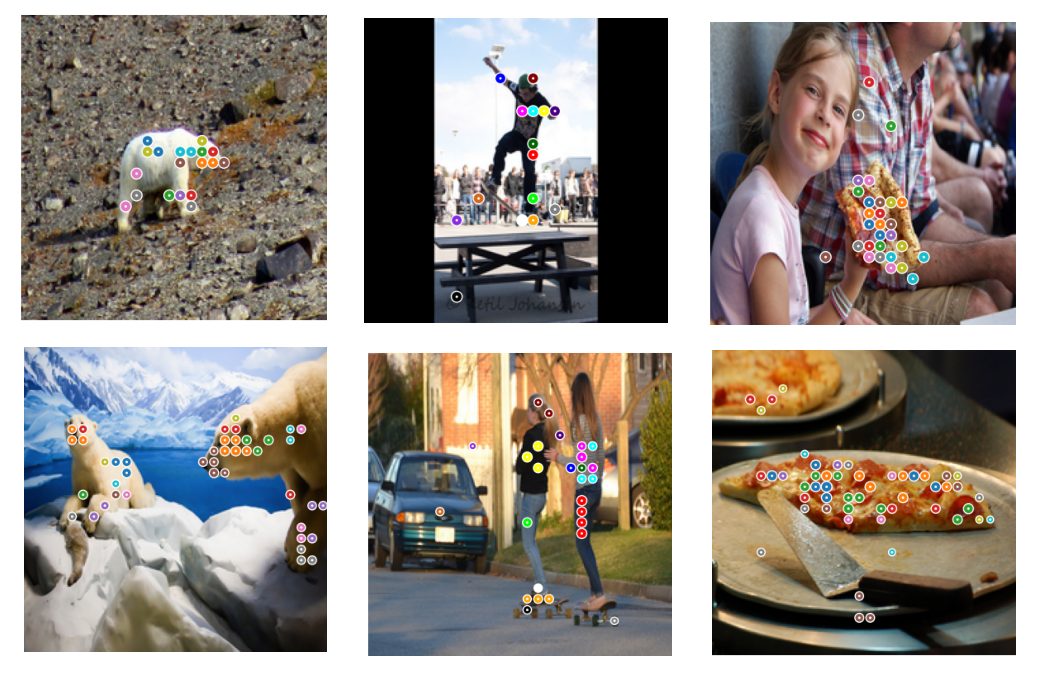
\includegraphics[width=0.95\textwidth]{Images/main/correspondences.png}
	\caption[\textbf{Keypoint Correspondences Using Relaxed Best Buddies}]{\textbf{Keypoint Correspondences Using Relaxed Best Buddies}. Prototype images at the top and query images at the bottom. Same colored points represent similar features }
	\label{fig:correspondecences}
\end{figure*}

For a good part of the thesis work, we worked with keypoint correspondences extracted from similarity matrix of key descriptors of two images to extract semantically similar parts in the image and use this information to separate the instances. We extracted the instances using keypoint correspondences taking inspiration from the Superglue~\cite{sarlin2020supergluelearningfeaturematching} paper. But the main challenge was instead of working with images taken two different perspectives, we are dealing with entirely different pair of images with similar instances.

Figure~\ref{fig:correspondecences} shows the keypoint correspondences between the prototype and query images. The correspondence is calculated by applying the relaxed best buddy algorithm on the descriptors corresponding to the foreground part of the prototype and query images, which is selected by applying a threshold on the saliency map. We relaxed the original best buddy algorithm~\cite{Aberman_2018} to extract more correspondence points enough to form a graph to perform graph-cut similar to~\cite{wang2022tokencut, sarlin2020supergluelearningfeaturematching}. We explored our options to geometrically separate the instances using the semantic information in the correspondences. But as we were unable to find a promising approach or inspiration from our research. For instance, Integer programming for multidimensional assignment problem~\cite{WALTEROS2014553} has a strict initial graph specification which restrict us to adapt it to our problem.

By considering the limitations of implementing a semi-supervised method using keypoint correspondences, we focused mostly on improving the unsupervised instance detection and segmentation by diving into the current state-of-the-art method CutLER~\cite{wang2023cut}; exploring it's limitations and ways to improve them. Nevertheless we recognize the potential of leveraging keypoint correspondences for instance detection and believe this approach warrants further exploration in future research.

\subsection{Sensitivity to Hyperparameters}
The MaskCut and mask filtration processes within the CutLER framework are highly dependent on various hyperparameters, such as the theshold for maximum number of masks generated in MaskCut, IoU threshold for mask selection and the confidence score used to filter pseudo-ground truths. These hyperparameters play a crucial role in determining the quality of the masks and, consequently, the overall performance of the model in unsupervised instance detection and segmentation tasks.

Investigating the potential of adaptive or dynamic hyperparameter tuning, where the model adjusts these values during training based on performance metrics, could lead to more robust and generalized mask generation. Such future work would help in further refining the CutLER framework and potentially extend its applicability across a broader range of datasets and tasks.

\subsection{Unsupervised Detection of Overlapping Instances}
Based on our findings, a key area for future research will be the development of unsupervised methods designed to better detect both individual and overlapping instances within images. It would be beneficial to extend our approach beyond merely filtering out images with overlapping instances. Developing techniques to further separate and identify individual instances within these overlapping regions could address a significant challenge in unsupervised learning. Given that many unsupervised methods currently struggle with distinguishing overlapping instances, this direction holds promise for enhancing the accuracy and robustness of instance detection and segmentation in complex scenarios.


%GroupViT introduced a fresh perspective to semantic segmentation through a bottom-up approach. We closely examined GroupViT to grasp its two fundamental ideas: Grouping and Recognition. We then assessed each of these concepts individually to identify opportunities for improvement. We systematically pursued these enhancements to develop an efficient fine-tuning strategy.
%
%
%During our investigation, we thoroughly analyzed various aspects of training and refining the text extraction process. To enhance our approach, we further introduced entropy regularization techniques. When our model is trained on high-resolution images, these techniques not only improve mIoU on the training dataset but also have a positive impact on downstream dataset performance.
%
%In our pursuit of enhancing the model's performance further, we integrated a noise-free contrastive loss tailored for training on a cleaner, smaller dataset like MSCOCO. By following this recipe of fine-tuning, we witnessed an increase of  18\% mIoU on the COCO dataset, all while maintaining consistent performance on other datasets such as PASCAL VOC and PASCAL Context.
%
%Furthermore, we investigated the potential of utilizing GroupViT's grouping mechanism for grouping DINO features. In addition, we made progress in the direction of knowledge distillation from DINO to GroupViT by introducing a formulation, establishing a foundation for potential advancements in this area.
%
%In essence, our exploration of GroupViT has involved dissecting its components, refining its training process while maintaining its capabilities on downstream datasets, and delving into opportunities for knowledge distillation. This journey has not only revealed the intricacies of GroupViT but also pointed toward promising directions for future advancements.
%\section{Future Work}
%
%The future possibilities for advancing GroupViT's capabilities present an exciting journey. We provide a brief overview of these prospects here:
%
%\subsection{Integration of DINO Features: Synergizing Strengths}
%A promising direction for future exploration involves integrating DINO and GroupViT. This integration would involve developing a unified framework to compare deep-layer features extracted from DINO and segment features extracted from GroupViT within a shared context. Additionally, investigating the potential of knowledge distillation could unveil new opportunities for enhancing the model's visual grouping capabilities..
%
%\subsection{Enriching Negative Sample Pool for Noise-Free Contrastive Loss}
%While the advantages of noise-free contrastive loss are clear, we must address the challenge of a limited negative sample pool. An effective approach to overcome this challenge is the creation of an extensive memory bank for negative samples. By this, the model can benefit from noise-free contrastive loss while maintaining a diverse set of negative samples, potentially resulting in enhanced performance.
%
%\subsection{Exploring Hierarchical Grouping with Web-Scaled Data}
%The potential of hierarchical grouping at more advanced stages remains unexplored due to resource limitations in our study. Expanding this research to include web-scaled datasets could provide valuable insights into the impact of hierarchical grouping on advanced stages of GroupViT.
%
%\subsection{Training with Datasets Including Stuff Classes}
%While GroupViT performs well on datasets like Pascal VOC and MSCOCO, it encounters difficulties with more complex datasets such as Context and ADE20K. These challenges arise from the presence of stuff classes like `air', `water', and `sky', which are relatively underrepresented in human-annotated datasets like MSCOCO. To tackle this issue, future efforts could involve training GroupViT on datasets explicitly designed to include these stuff classes or specialized datasets created for this purpose. This approach has the potential to enhance GroupViT's adaptability to real-world scenarios and improve its performance across diverse scenes. 
%
